\documentclass[12pt,a4paper]{article}
\usepackage{bm}
\usepackage{longtable}
\def\toP{\xrightarrow{\P}}
\def\tod{\xrightarrow{\mathrm{d}}}

\ifxetex
\defaultfontfeatures{Ligatures={TeX},Renderer=Basic}
\usepackage{libertine}
\setmainfont[
  Ligatures=TeX,
  Extension         = .otf,
  BoldFont          = LinLibertine_RZ,
  ItalicFont        = LinLibertine_RI,
  BoldItalicFont    = LinLibertine_RZI,
]{LinLibertine_R}
\setdefaultlanguage{russian}  %% устанавливает главный язык документа
\setotherlanguage{english}
\setmathfont{xits-math.otf}
\setmathfont[range={\mathcal,\mathbfcal},StylisticSet=1]{xits-math.otf}
\else
\fi

\usepackage[left=2cm,right=2cm,top=2cm,bottom=2cm]{geometry}
\parindent=1cm
        % Подключаемые пакеты
\ifxetex
\defaultfontfeatures{Ligatures={TeX},Renderer=Basic}
\usepackage{libertine}
\setmainfont[
  Ligatures=TeX,
  Extension         = .otf,
  BoldFont          = LinLibertine_RZ,
  ItalicFont        = LinLibertine_RI,
  BoldItalicFont    = LinLibertine_RZI,
]{LinLibertine_R}
\setdefaultlanguage{russian}  %% устанавливает главный язык документа
\setotherlanguage{english}
\setmathfont{xits-math.otf}
\setmathfont[range={\mathcal,\mathbfcal},StylisticSet=1]{xits-math.otf}
\else
\fi

\usepackage[left=2cm,right=2cm,top=2cm,bottom=2cm]{geometry}
\parindent=1cm
          % Пользовательские стили

\newcommand{\then}{\ \Longrightarrow \ }
\newcommand{\eps}{\varepsilon}
\newcommand{\com}{\backslash \backslash}
\renewcommand{\C}{\mathbb{C}}
\newcommand{\E}{\mathbb{E}}
\newcommand{\D}{\mathbb{D}}
\renewcommand{\P}{\mathbb{P}}
\newcommand{\R}{\mathbb{R}}
\newcommand{\Q}{\mathbb{Q}}
\newcommand{\Z}{\mathbb{Z}}
\newcommand{\N}{\mathbb{N}}
\newcommand{\vphi}{\varphi}
\newcommand{\iaoi}{\ \Longleftrightarrow \ }
\newcommand{\empt}{\varnothing}
\newcommand{\A}{\mathfrak{A}}
\newcommand{\sm}{\sum\limits}
\newcommand{\I}{\mathbb{I}}
\renewcommand{\it}{\int\limits}
\renewcommand{\L}{\mathcal{L}}
\renewcommand{\bar}{\overline}
\renewcommand{\tilde}{\widetilde}

\newtheorem*{thmnn}{Теорема}
\newtheorem*{thm}{Теорема}
\newtheorem*{dfn}{Определение}
\newtheorem*{sug}{Предложение}
\newtheorem*{prop}{Свойство}
\newtheorem*{lem}{Лемма}
\newtheorem*{con}{Следствие}
\newtheorem*{note}{Замечание}
\newtheorem{exer}{Задача}
\newtheorem*{notation}{Напоминание}
\newtheorem*{ex}{Пример}
\newtheorem*{design}{Обозначение}

\ifxetex
\newcommand{\mathbbold}{\mathbb}
\else
\DeclareMathAlphabet{\mathbbold}{U}{bbold}{m}{n}
\fi

\DeclareMathOperator{\ord}{ord}
\DeclareMathOperator{\val}{val}
\DeclareMathOperator{\rk}{rk}
\DeclareMathOperator{\cov}{cov}
\DeclareMathOperator{\cor}{cor}
\DeclareMathOperator{\diag}{diag}

\DeclareMathOperator*{\argmin}{arg\,min}
\DeclareMathOperator*{\argmax}{arg\,max}


\newcommand{\Tr}[1]{#1^{\mathrm{T}}}


\newcommand{\Inner}[2]{\langle\,#1, #2\,\rangle}

\newcommand{\Outer}[2]{ #1\otimes#2}


\newcommand{\Header}{
  \begin{center}
    {\Large\bf
     Многомерный анализ данных: классификация и кластерный анализ
     
         \vspace{0.7em}
     для магистров СПбГУ, ПМИ, статмод
      }
      
    \vspace{0.7em}
      {Голяндиной Н.Э. (черновой вариант, просьба сообщать об опечатках)
      
     \vspace{20cm} 
          Первоначальный набор теста --- выпуск статмода 2017 (магистратура)
      }\\


    \vspace{0.7em}
    {Собрано {\today} в {\currenttime}}
  \end{center}

  \vspace{1em}
  %\tableofcontents
  \pagebreak
}


\begin{document}
\Header
      \section{Классификация}
\subsection{Общий подход к классификации через апостериорные вероятности} % (fold)
	Общая подход к классификации: строятся классифицирующие функции $f_i$, такие что классификация проводится так:
индивид с признаками $\mathbf{x}$ относится к группе с максимальным значением на нем классифицирующей функции:
$\argmax_i\mathrm f_i(\mathbf{x})$.

 Откуда берутся эти классифицирующие функции? Естественная идея взять в качестве $f_i$ вероятность (ее оценку)
принадлежности к $i$-му классу.
Пусть $\xi$ -- дискретная с.в., принимающая значения $\left\lbrace A_i\right\rbrace_{i=1}^k$, $\mathcal P(\eta\mid \xi = A_i) = \mathcal P_i$ и имеет плотность $p_i(\mathbf{x})$. Тогда было бы логично взять $f_i = p_i$. Для практического применения надо было бы оценить плотности, либо непараметрически (например, по числу точек, попавших в дельта-окрестность --- типа метода ближайших соседей), либо параметрически (если известно, что распределение нормальное, тогда просто оцениваем векторы средних и ковариационные матрицы).

Более сложный подход --- через апостериорные вероятности. Если у нас есть априорное знание вероятности того, что индивид
из того или иного класса, то мы можем его учесть.
Введем понятие класса $C_i = \left\lbrace\xi = A_i\right\rbrace$.  Чтобы классифицировать наблюдение $\mathbf{x}$, необходимо найти
	$$\argmax\mathrm P\left(\xi = A_i\middle\vert \eta = \mathbf{x}\right) = \argmax\mathrm P\left(C_i\middle\vert \mathbf{x}\right).$$

	Пусть известны априорные вероятности принадлежности нового наблюдения к $i$-му классу $\pi_i = \mathrm P\left(C_i\right)$. Тогда апостериорные вероятности по формуле Байеса будут иметь вид $$\mathrm P\left(C_i\middle\vert \mathbf{x}\right) = \frac{\mathrm P\left(\mathbf{x}\middle\vert C_i\right) \pi_i}{\sum_{j=1}^k \mathrm P\left(\mathbf{x}\middle\vert C_j\right) \pi_j}.$$
Поэтому в качестве классифицирующих функций берут
$$f_i\left(\mathbf{x}\right) = \frac{p_i(\mathbf{x}) \pi_i}{\sum_{j=1}^k p_j(\mathbf{x}) \pi_j}. $$

	Так как знаменатель у всех $f_i$ одинаковый, его можно отбросить, и итоговые классифицирующие функции будут выглядеть как $f_i\left(\mathbf{x}\right) = \mathrm P\left(\mathbf{x}\middle\vert C_i\right) \pi_i = p_i(\mathbf{x}) \pi_i$.

	Как выбрать априорные вероятности?

	\begin{enumerate}
		\item Равномерно, $\forall i \in 1\mathbin : k \; \pi_i = 1 \mathbin / k$.
		\item По соотношениям в обучающей выборке: $\pi_i = n_i \mathbin / \sum_{j=1}^k n_j$.
		\item На основе другой дополнительной информации о данных (результаты предыдущих исследований, etc.)
	\end{enumerate}

\begin{prop}
Построенный метод классификации $\mathrm{predict}(\mathbf{x}) = \argmax_i \pi_i p_i(\mathbf{x})$ минимизирует среднюю апостериорную ошибку:
$$\sum_{i=1}^k \pi_i \mathrm P(\mathrm{predict}(\mathbf{x}) != i\mid C_i).$$
\end{prop}

Видно, что можно с помощью априорных вероятностей формально задавать важность ошибочных классификаций
для разных классов.

%\end{document}
\subsection{Линейный и квадратичный дискриминантный анализ для классификации}
	\subsubsection{LDA} % (fold)
	\label{ssub:lda}
		Модель: $\xi$ --- дискретная с.в., принимающая значения $\left\lbrace A_i\right\rbrace_{i=1}^k$, $\mathcal P(\eta\mid \xi = A_i) = \mathcal N\left(\bm{\mu}_i, \bm{\Sigma}\right)$. Тогда плотность в точке $\mathbf{x}$
		$$p_i(\mathbf{x}) = p\left(\mathbf{x}\middle\vert \xi = A_i\right) = \frac{1}{\left(2\pi\right)^{p/2}\left\vert\bm{\Sigma}\right\vert^{1/2}} \exp\left(-\frac{1}{2}\Tr{\left(\mathbf{x} - \bm{\mu}_i\right)}\bm{\Sigma}^{-1}\left(\mathbf{x} - \bm{\mu}_i\right)\right),$$
		и классифицирующая функция $f_i\left(\mathbf{x}\right) = \pi_i p\left(\mathbf{x}\middle\vert \xi = A_i\right)$, где $\pi_i$ --- априорная вероятность наблюдения попасть в $i$-ю группу. Для упрощения вычислений можно переписать классифицирующую функцию через возрастающее монотонное преобразование как

		$$g_i\left(\mathbf{x}\right) = \log f_i\left(\mathbf{x}\right) = \log \pi_i - \frac{1}{2}\log\left\vert\bm{\Sigma}\right\vert -  \frac{1}{2}\Tr{\left(\mathbf{x} - \bm{\mu}_i\right)}\bm{\Sigma}^{-1}\left(\mathbf{x} - \bm{\mu}_i\right).$$
Сократив часть, не зависящую от номера класса, получаем линейные классифицирующие функции
$$h_i(\mathbf{x}) = -\frac{1}{2}\Tr{\bm{\mu}_i}\bm{\Sigma}^{-1}\bm{\mu}_i + \Tr{\bm{\mu}_i}\bm{\Sigma}^{-1}\mathbf{x} + \log\pi_i.$$

\begin{note}
  Если две группы, то гипотеза о равенстве многомерных мат.ож. $H_0: \bm{\mu}_1 = \bm{\mu}_2$ (различие значимо, если гипотеза отвергается, а только тогда имеет смысл проводить классификацию) в модели LDA проверяется с помощью критерия Хотеллинга (Hotelling). Если групп несколько, то есть разные критерии, например, критерия Wilk's Lambda или Roy's greatest root (эти же критерии используются в MANOVA, Multivariate ANalysis Of VAriance). Они отличаются мощностью против разного расположения групп.
\end{note}

\paragraph{Немного про канонические переменные}
В LDA есть так называемые канонические переменные. Идея похожа на АГК, только оптимизационная задача другая. Аналогично, на основе исходных признаков (признаки центрируются) строятся новые признаки как линейные комбинации исходных признаков. Только первая каноническая переменная --- это такая линейная комбинация исходных признаков, по которой группа максимально отличаются (отличие измеряется на основе ANOVA, по статистике критерия Фишера). Вторая линейная комбинация должна быть ортогональна первой и приводит к максимальному различию среди ортогональных линейных комбинаций. И т.д. Удобно смотреть на данные в плоскости первой и второй канонических переменных (иногда это называют roots).

\medskip
Приведем формулу, как находятся коэффициенты линейной комбинации (канонические коэффициенты) для получения канонических переменных. Неудивительно, что экстремальная задача приводит к поиску собственных векторов некоторой матрицы.

Имеет место разложение выборочной ковариационной матрицы, умноженной на $n$ (индивид $\mathbf y_{ij} \in \R^p$ --- $j$-й индивид из $i$-й группы):
\begin{gather}
    \label{VI_MANOVA}
    \sum_{i=1}^k \sum_{j=1}^{n_i} (\mathbf y_{ij} - \overline {\mathbf y}) \Tr{(\mathbf y_{ij} - \overline {\mathbf y})} =
    \sum_{i=1}^k n_i (\overline {\mathbf y_i} - \overline {\mathbf y}) \Tr{(\overline {\mathbf y_i} - \overline {\mathbf y})} +
    \sum_{i=1}^k \sum_{j=1}^{n_i} (\mathbf y_{ij} - \overline {\mathbf y_i}) \Tr{(\mathbf y_{ij} - \overline {\mathbf y_i})}
    = \mathbf{H}  + \mathbf{E}.
\end{gather}
Должно быть ясно, что это лишь многомерное обобщение разложения выборочной дисперсии (умноженной на $n$).

Первое слагаемое отвечает за равенство средних (неотличимые группы), его назовем $\mathbf{H}$ от слов hypothesis, а второе --- за отклонение данных в каждой группе от своего среднего, его назовем $\mathbf{E}$ от слова error.

В этих обозначениях, канонические коэффициенты являются собственными векторами матрицы $\mathbf{E}^{-1}\mathbf{H}$. А собственные числа $\lambda_i$ (упорядоченные по убыванию вместе с собственными векторами) этой матрицы отражают то, насколько группы хорошо разделяются по соответствующей канонической переменной. Число ненулевых собственных чисел $s\le \min(n, k-1)$.

Критерии для проверки гипотезы о том, что группы не разделимы ($H_0:\bm\mu_1=\ldots=\bm\mu_k$), являются комбинацией этих собственных чисел. Например, статистика критерия Wilks' Lambda $$\Lambda = \prod_{i=1}^s {\frac{1}{1 + \lambda_i}}$$ (с какой стороны критическая область?). А статистика критерия Roy's greatest root имеет вид $$r_1^2 = \frac{\lambda_1}{1+\lambda_1} $$ (с какой стороны критическая область?).

Как понять, против какого расположения группы мощнее один, а против какого --- другой?
	% subsubsection lda (end)

	\subsubsection{QDA} % (fold)
	\label{ssub:qda}

	Модель: $\xi$ --- дискретная с.в., принимающая значения $\left\lbrace A_i\right\rbrace_{i=1}^k$, $\mathcal P(\eta\mid \xi = A_i) = \mathcal N\left(\bm{\mu}_i, \bm{\Sigma}_i\right)$. Тогда плотность в точке $\mathbf{x}$
		$$p\left(\mathbf{x}\middle\vert \xi = A_i\right) = \frac{1}{\left(2\pi\right)^{p/2}\left\vert\bm{\Sigma}_i\right\vert^{1/2}} \exp\left(-\frac{1}{2}\Tr{\left(\mathbf{x} - \bm{\mu}_i\right)}\bm{\Sigma}_i^{-1}\left(\mathbf{x} - \bm{\mu}_i\right)\right),$$
		и классифицирующая функция $f_i\left(\mathbf{x}\right) = \pi_i p\left(\mathbf{x}\middle\vert \xi = A_i\right)$. Применяем возрастающее монотонное преобразование и оставляем в классифицирующей функции только члены, отличающиеся в разных группах:

		$$g_i\left(\mathbf{x}\right) = \log f_i\left(\mathbf{x}\right) = \log \pi_i - \frac{1}{2}\log\left\vert\bm{\Sigma}_i\right\vert -  \frac{1}{2}\Tr{\left(\mathbf{x} - \bm{\mu}_i\right)}\bm{\Sigma}_i^{-1}\left(\mathbf{x} - \bm{\mu}_i\right),$$
получаем квадратично зависящую от $\mathbf{x}$ классифицирующую функцию.

\begin{note}
  Если две группы, то гипотеза о равенстве многомерных мат.ож. $H_0: \bm{\mu}_1 = \bm{\mu}_2$ (различие значимо, если гипотеза отвергается, а только тогда имеет смысл проводить классификацию) в модели QDA тоже проверяется с помощью критерия Хотеллинга (Hotelling), но с отдельно оцененными ковариационными матрицами (критерий асимптотический). Если групп несколько, то тут уже критерий сложно построить.
\end{note}

\newpage
\subsection{Классификация в случае двух классов}
Если всего два класса, то можно построить границу между классами, приравняв классифицирующие функции.
\subsubsection{LDA} % (fold)
Приравняв $h_1(x)= h_2(x)$, получим разделяющую гиперплоскость.
Разделяющая два класса гиперплоскость имеет вид
\begin{multline*}
  \{\mathbf{x} : h_1(\mathbf{x}) = h_2(\mathbf{x})\} =\\ = \{\mathbf{x} : -\frac{1}{2} (\bm{\mu}_1 - \bm{\mu}_2)^\mathrm{T} \mathbf{\bm{\Sigma}}^{-1}(\bm{\mu}_1 + \bm{\mu}_2) + (\bm{\mu}_1 - \bm{\mu}_2)^\mathrm{T} \mathbf{\bm{\Sigma}}^{-1}\mathbf{x} + \log(\pi_1/\pi_2) = 0\}.
\end{multline*}
От соотношения между априорными вероятностями зависит положение границы относительно классов (к какому она ближе).
Видно, что априорные вероятности влияют только на сдвиг разделяющей гиперплоскости.

Заметим, что классификацию можно записать как сравнение $-\frac{1}{2} (\bm{\mu}_1 - \bm{\mu}_2)^\mathrm{T} \mathbf{\bm{\Sigma}}^{-1}(\bm{\mu}_1 + \bm{\mu}_2) + (\bm{\mu}_1 - \bm{\mu}_2)^\mathrm{T} \mathbf{\bm{\Sigma}}^{-1}\mathbf{x}$ с некоторым порогом ($-\log(\pi_1/\pi_2)$), который зависит от априорных вероятностей
(или весов ошибок для разных классов, смотря как на это смотреть).

\subsubsection{QDA} % (fold)
	В данном случае, разделяющая поверхность имеет вид квадратичной поверхности, может состоять из двух гиперболоидом,
может иметь форму эллипса.

\subsubsection{Картинки}

	\begin{figure}[!h]
		%\subfigure{
			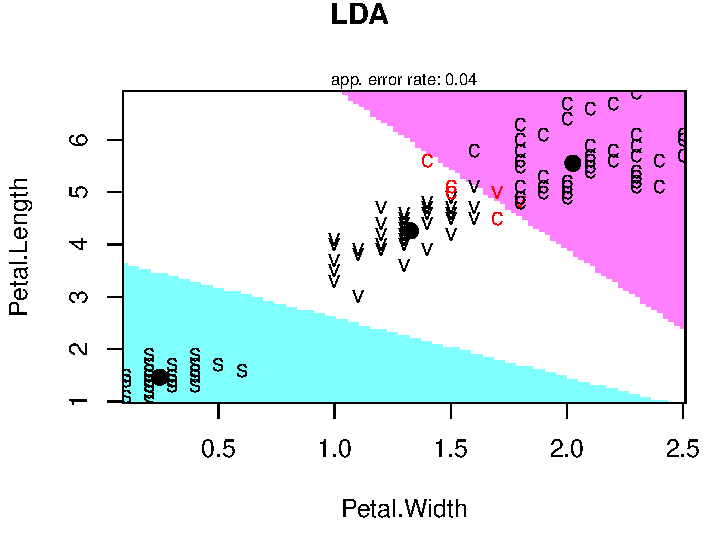
\includegraphics[width=0.5\textwidth]{img/lda.pdf}
			\includegraphics[width=0.5\textwidth]{img/qda.pdf}\\
			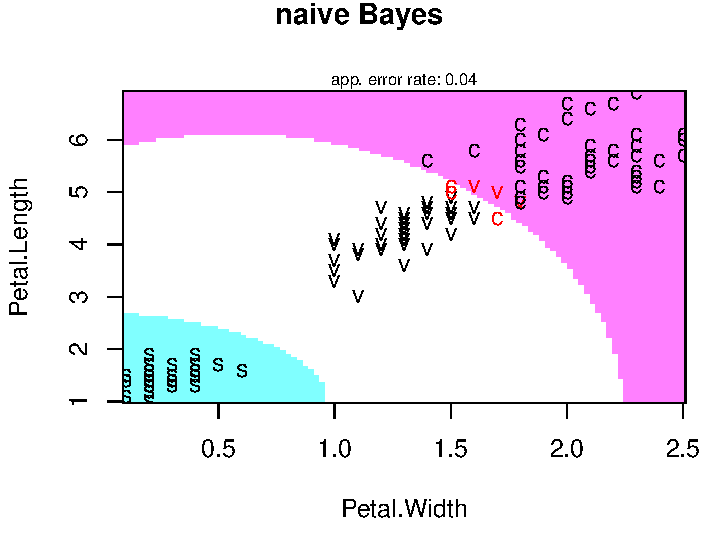
\includegraphics[width=0.5\textwidth]{img/nbda.pdf}
			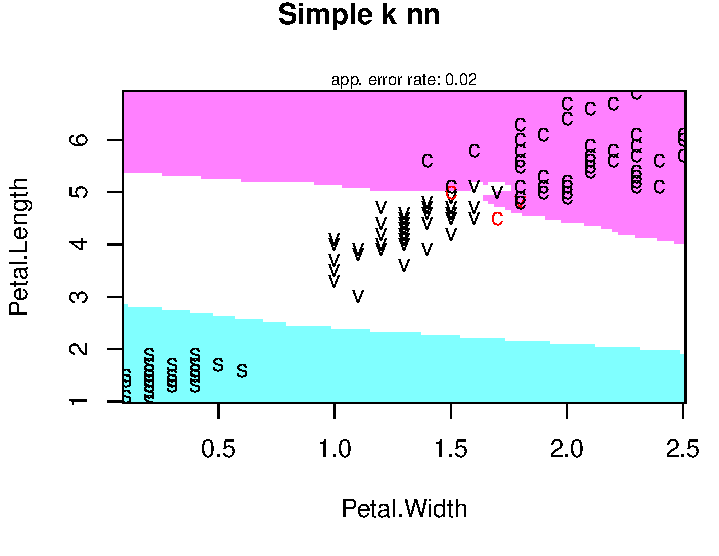
\includegraphics[width=0.5\textwidth]{img/sknn.pdf}
		%}
	\end{figure}

Здесь мы обсуждали число параметров в моделях, возможный overfitting (переподгонку).
Использовали слова --- обобщающая способность алгоритма.

\subsection{Качество классификации}


\subsubsection{Ошибки класификации}

Качество классификации измеряется ошибками классификации (доля неправильно классифицированных объектов).
$n_{ij}$ --- число объектов из класса $i$, отнесенных к классу $j$. В соответствующей матрице классификации
на диагонали стоят правильно классифицированные объекты, вне диагонали --- ошибки.

На самом деле, нельзя проверять качество предсказания на тех данных, на которых это предсказание строилось.
Поэтому используют кросс-валидацию (скользящий контроль).
Например, каждое наблюдение по очереди исключается из выборки, классифицирующее правило строится без него и с
 помощью этого правила индивид классифицируется. Строится аналогичная таблица из $n_{ij}$. В ней ошибок будет,
 вообще говоря, больше.

 Здесь обсуждали, что имеет смысл смотреть на ошибки без кросс-валидации и с ней. Если разница существенная, то
 это говорит о переподгонке используемой модели. Вероятно, она не очень хорошая; например, слишком много
 параметров.

Замечание. Нельзя путать классификацию и различие групп. Группы могут значимо различаться, классификация может
быть при этом бессмысленной
(ошибок чуть меньше 50\%).

\subsubsection{ROC и AUC}

\paragraph{wikipedia}

ROC-кривая (англ. receiver operating characteristic, рабочая характеристика приёмника) --- график, позволяющий оценить качество бинарной классификации, отображает соотношение между долей объектов от общего количества носителей признака, верно классифицированных как несущих признак, (англ. true positive rate, TPR, называемой чувствительностью алгоритма классификации) и долей объектов от общего количества объектов, не несущих признака, ошибочно классифицированных как несущих признак (англ. false positive rate, FPR, величина 1-FPR называется специфичностью алгоритма классификации) при варьировании порога решающего правила.

Также известна как кривая ошибок. Анализ классификаций с применением ROC-кривых называется ROC-анализом.

Количественную интерпретацию ROC даёт показатель AUC (англ. area under ROC curve, площадь под ROC-кривой) — площадь, ограниченная ROC-кривой и осью доли ложных положительных классификаций. Чем выше показатель AUC, тем качественнее классификатор, при этом значение 0,5 демонстрирует непригодность выбранного метода классификации (соответствует случайному гаданию). Значение менее 0,5 говорит, что классификатор действует с точностью до наоборот: если положительные назвать отрицательными и наоборот, классификатор будет работать лучше.

\paragraph{мои комментарии}

Если кто-то хорошо представляет себе, как выглядит график зависимости мощности от ошибки первого рода, то это именно такой график.
Меняется уровень значимости (как порог отвергнуть - не отвергнуть) и по оси x откладывается ошибка первого рода, она же false positive rate FP/(TN+FP), а по оси y откладывается
мощность, она же true positive rate TP/(TP+FN)(слово positive означает, что нулевая гипотеза отвергнута в пользу второй, альтернативной, гипотезы,
а в случае классификации, что элемент классифицируется как относящийся ко второму классу).

Таким образом, меняем порог/параметр для метода классификации (пример параметра --- априорная вероятность $\pi_1$)
и по оси x откладываем долю неправильно классифицированных элементов из первого класса ($n_{12}/(n_{11}+n_{12})$, FPR),
а по оси y --- долю правильно классифицированных элементов из второго класса ($n_{22}/(n_{22}+n_{21})$, TPR).

\includegraphics[width=10cm]{img/expl_roc}

Пусть классы имеют вид $4,6,8,10,12$ первый и $1,3,5,7$ второй. Опишем ROC-кривую. Пусть к первому классу мы относим, если число больше порога $\gamma$. Для $\gamma < 1$ мы находимся в точке $(0, 0)$. При $1 < \gamma < 3$ мы перескакиваем в точку $(0, 0.25)$. При $3 < \gamma < 4$ мы перескакиваем в точку $(0, 0.5)$. При $4 < \gamma < 5$ мы перескакиваем в точку $(0.2, 0.5)$. При $5 < \gamma < 6$ мы перескакиваем в точку $(0.2, 0.75)$.
При $6 < \gamma < 7$ мы перескакиваем в точку $(0.4, 0.75)$. При $7 < \gamma < 8$ мы перескакиваем в точку $(0.4, 1)$. Дальше мы при $x=1$ последовательно перескакиваем по $y$ в 0.6, 0.8 и при $\gamma >12$ попадаем в точку $(1,1)$.



%\end{document}
	% subsubsection qda (end)


% subsection _30_ (end)

	
      %\subsection{Билет 41 Объясненные	каноническими	переменными	доли	дисперсии.	Избыточность.}
%Пусть $\overline{\xi} \in \R^p, \ \overline{\eta} \in \R^q$ --- исходные признаки.
%$A_i^T \overline{\xi}, \ B_i^T \overline{\eta}$ --- $i$-ые канонические направления.
%Утверждается, что, если $\mathbb{E}\xi_i = 0, \mathbb{D}\xi_i = 1, \ \mathbb{E}\eta_i = 0, \mathbb{D}\eta_i = 1 \ \forall i$, то
%\begin{equation*}
%\sum\limits_{k = 1}^{s} \rho^2(\eta_i, B_k^T \overline{\eta}) \le 1 = \mathbb{D}\eta_i, \ \sum\limits_{k = 1}^{s} \rho^2(\xi_i, A_k^T \overline{\xi}) \le 1 = \mathbb{D} \xi_i , \ s = \min(p, q).
%\end{equation*}
%При этом, если $s = q$, то в первом случае достигается равенство, а если $s = p$, то во втором.
%Поэтому $\sum\limits_{k = 1}^{s} \rho^2(\eta_i, B_k^T \overline{\eta})$ и $\sum\limits_{k = 1}^{s} \rho^2(\xi_i, A_k^T \overline{\xi})$ называется объясненной долей дисперсии.
%
%\textbf{Избыточность:}
%Избыточностью $i$-ого левого признака $\xi_i$ называется
%\begin{equation*}
%\sum\limits_{k = 1}^{s} \rho^2(\xi_i, B_k^T \overline{\eta}).
%\end{equation*}
%Аналогично для правых. На консультации мы не разобрались, как ее интерпретировать, поэтому достаточно только определения.

%\subsection{Билет 42.Что общего	между	дискриминантным	анализом в многомерной	множественной	регрессией?}
%Окей, давайте по порядку.
%Задача MANOVA (буду сразу писать в нормальной модели с равными ковариационными матрицами, а не начинать с общей задачи на равенство распределений):
%
%Пусть $\eta_i \sim \mathcal{N}(\mu_i, \Sigma)$, $i = 1, \ldots k$.
%
%Необходимо проверить гипотезу
%\begin{equation*}
%H_0: \mu_1 = \ldots = \mu_k.
%\end{equation*}
%Введем одномерный качественный признак $\xi$, принимающий значения $A_1, \ldots A_k$. Тогда можно рассмотреть пару $(\eta, \xi)$, такую что $\mathcal{P}_{\eta \mid \xi = A_i} = \mathcal{P}_{\eta_i}$ и гипотеза принимает вид
%\begin{equation*}
%H_0: \mathbb{E}(\eta \mid \xi = A_1) = \ldots = \mathbb{E}(\eta \mid \xi = A_k).
%\end{equation*}
%Что эквивалентно независимости $\eta$ от $\xi$
%Знаем, что
%\begin{equation*}
%\mathbb{E}(\eta - \mathbb{E}\eta)(\eta - \mathbb{E}\eta)^T = \mathbb{E}(\mathbb{E}(\eta \mid \xi) - \mathbb{E}\eta)(\mathbb{E}(\eta \mid \xi) - \mathbb{E}\eta)^T + \mathbb{E}(\eta - \mathbb{E}(\eta \mid \xi))(\eta - \mathbb{E}(\eta \mid \xi))^T
%\end{equation*}
%То есть, на самом деле мы можем проверять гипотезу о том, что
%\begin{equation*}
%H_0: \mathbb{E}(\mathbb{E}(\eta \mid \xi) - \mathbb{E}\eta)(\mathbb{E}(\eta \mid \xi) - \mathbb{E}\eta)^T = 0
%\end{equation*}
%Теперь перейдем на выборочный язык и напишем основное дисперсионное тождество ($n_i$ -- длина выборки для $i$-ой группы.
%\begin{equation*}
%\sum\limits_{i = 1}^{k}\sum\limits_{j = 1}^{n_i}(y_{ij} - \overline{y})^2 = \sum\limits_{i = 1}^{k}n_i(y_{ij} - \overline{y}_{i.})^2  + \sum\limits_{i = 1}^{k}\sum\limits_{j = 1}^{n_i}(\overline{y}_{i.} - \overline{y})^2 = \mathbf{H} + \mathbf{E}
%\end{equation*}
%Статистика критерия, проверяющая нашу гипотезу имеет вид
%\begin{equation}
%\Lambda = \frac{|\mathbf{E}|}{|\mathbf{E} + \mathbf{H}|} = \prod\limits_{i = 1}^s (\frac{1}{1 + \lambda_i}),
%\label{maov}
%\end{equation}
%где $\lambda_i$ -- собственные числа матрицы $\mathbf{E}^{-1} \mathbf{H}$, $s = \min(p, k-1).$
%
%Теперь введем переменные $\zeta_1, \ldots, \zeta_{k-1}$ как dummy variables для переменной $\xi$ и рассмотрим многомерную множественную линейную регрессию вектора $\overline{\zeta}$ на $\eta$.
%А именно рассмотрим
%\begin{equation*}
%\mathbf{Y} = \mathbf{X}\mathbf{B} + \Xi
%\end{equation*}
%Предположим, что $\mathbf{Y}$ и $\mathbf{X}$ --- центрированы.
%Решение данной задачи $\hat{\mathbf{B}} = (\mathbf{X}^T\mathbf{X})^{-1}\mathbf{X}^T \mathbf{Y}$.
%Значимость регрессии проверяется гипотезой
%\begin{equation*}
%H_0: \mathbf{B} = 0.
%\end{equation*}
%Положим $\mathbf{E} = (\hat{\mathbf{Y}} - \mathbf{Y})(\hat{\mathbf{Y}} - \mathbf{Y})^T$,
%$\mathbf{H} = \hat{\mathbf{Y}}\hat{\mathbf{Y}} ^T$ и статистика критерия имеет вид
%\begin{equation}
%\Lambda = \frac{|\mathbf{E}|}{|\mathbf{E} + \mathbf{H}|} = \prod\limits_{i = 1}^s \left(\frac{1}{1 + \lambda_i}\right) = \prod(1 - r^2_i),
%\label{regr}
%\end{equation}
%где $r_i$ --- это $i$-ая каноническая корреляция.
%Так вот, оказывается, что $\Lambda$ из \eqref{maov} совпадает с  $\Lambda$ из $\eqref{regr}$.
%Таким образом получается, что $i$-ая каноническая корреляция между наборами $\zeta_1, \ldots, \zeta_{k-1}$ и $\eta_1, \ldots, \eta_p$ выражается через собственные числа $\lambda_i$, полученные в результате дискриминантного анализа как
%\begin{equation*}
%r_i^2 = \frac{\lambda_i}{1 + \lambda_i}
%\end{equation*}
%\subsection{Билет 43.Две группы, использование	множественной линейной регрессии для классификации.}
%Все в тех же обозначениях положим $k = 2$. Таким образом у нас получается только одна dummy-переменная и мы можем рассмотреть регрессию $\eta_1, \ldots, \eta_p$ на $\zeta_1$.
%(Мы все перевернули, но это не смертельно ибо в канонических корреляциях все симметрично).
%В таком случае первая каноническая корреляция $r^2_1 = R(\zeta, \eta_1, \ldots, \eta_p)$ --- это выборочный коэффициент корреляции.
%
%\begin{thm}
%Канонические коэффициенты $A_1$ пропорциональны $B^{(c)}$, которые получены при решении регрессионной задачи и пропорциональны $\Sigma^{-1}(\mu_1 - \mu_2)$.
%\end{thm}
%Вообще это частично показывалось, но я так поняла, что это не нужно..
%\newpage
\subsection{Кластерный анализ}

Цель кластерного анализа --- разбить индивиды на кластеры, т.е., на группы, между которыми, в некотором смысле,
расстояние больше, чем между точками внутри. Задача не формализована и, можно сказать, плохо поставлены,
 поэтому решается плохо.

Вообще, кластерный анализ --- это `обучение без учителя'. Это означает, что вы не сможете формально проверить правильность результата.

Единственный вариант поставить задачу четко --- это предположить какую-то статистическую модель данных и в ней находить
параметры, например, по методу максимального правдоподобия  (model-based clustering).

Все остальные методы --- эвристические с плохо определенным (хорошо-плохо) результатом.

\subsection{Кластерный	анализ,	пример	model-based	подхода}

Предположим, что многомерная выборка --- неоднородная. Но в отличие от дискриминантного анализа у нас нет признака, объясняющего эту неоднородность, и задачей является ее выявить.
Тип классификации, когда есть модель, называется model-based clustering.
Например, пусть наша выборка из смеси $k$ нормальных распределений. Таким образом ее плотность имеет вид
\begin{equation}
p(x) = \pi_1 p(x, \mu_1, \Sigma_1) + \ldots + \pi_k p(x, \mu_k, \Sigma_k),
\end{equation}
где
\begin{equation}
p(x, \mu_i, \Sigma_i) = \frac{1}{(2\pi)^{p/2}\sqrt{|\Sigma_i|}}
\exp \left(-\frac{1}{2}(x - \mu_i)\Sigma_i^{-1}(x - \mu_i)^T \right)
\end{equation}
Эта задача решается методом максимального правдоподобия. Можно выписать функцию правдоподобия (выпишите),
но она имеет сложный вид и искать ее максимум по такому большому числу параметров очень непросто.
Для нахождения этого максимума используется так называемый ЕМ-алгоритма (Expectation - Maximization).
Мы не будем здесь его обсуждать.



\subsection{Кластерный	анализ: $k$-means,	$k$-means$++$}
Хотим искать кластеры $C_1, \ldots, C_k$ минимизируя следующий функционал
\begin{equation}
\sum\limits_{i = 1}^k \sum\limits_{j \in C_i} ||x_j - \mu_i||^2
\label{func_lin}
\end{equation}
по разбиению всего пространства индивидов на $C_j$ и по всем $\mu_i$.
Можно делать это по следующему алгоритму:
\begin{enumerate}
\item Выбираем случайно $\mu_1, \ldots, \mu_k$.
\item $C_j$ -- кластер, содержащий точки, которые лежат к $\mu_j$ ближе, чем к остальным $\mu_i$.
\item Для каждого $C_j$ пересчитываем центр $\mu_j$ как выборочное среднее элементов из этого кластера.
\item Делаем 2 и 3 пока алгоритм не сойдется.
\end{enumerate}



\medskip
Проблема метода в том, что у такого функционала много локальных минимумов, и алгоритм может сойтись в значение, далекое от истинного.
Метод $k$-means$++$ повторяет алгоритм, приведенный выше, но начальные значения выбираются не случайно, а следующим образом
\begin{enumerate}
\item Выбираем случайным образом первый центр $\mu_1$.
\item Считаем расстояние от всех точек до ближайшего центра $\{\rho_i\}$. После чего выбираем $x_i$ как новый центр с вероятностью, пропорциональной $\rho_i$.
\item Пока количество центров меньше, чем $k$, повторяем процедуру.
\end{enumerate}
Результат функционала в $k$-means для данной процедуры выбора начальных центров запишем как $J(\{C_j\}, \{\mu_j\})$.
Известно, что при некоторых условиях на форму кластеров
\begin{equation*}
\frac{\mathbb{E}(J(\{C_j\}, \{\mu_j\}))}{J_{min}} = O(\ln k ),
\end{equation*}
т.е. результат, в среднем, довольно близко к настоящему минимуму.
%\subsection{Запись задачи, решаемой k-means, как задачи low-rank approximation с	ограничениями. Использование АГК}
%Функционал вида \eqref{func_lin} можно переписать в виде
%\begin{equation}
%    ||\mathbf{X} - \mathbf{G}\mathbf{M}||^2_F,
%\end{equation}
%где $M = (\mathbf{m}_1, \ldots, \mathbf{m}_k)$, $\mathbf{G}$ --- матрица, у которой в каждой строке
%стоит ровно одна единица и остальные нули.
%При этом, ранг матрицы $\mathbf{G}\mathbf{M}$ не превосходит $k$, что приводит нас к задачи
%аппроксимации заданной матрицы матрицей меньшего ранга.  Заметим, что задача похоже на задачу
%сингулярного разложения с ограничениями %\footnote{Матрица $\mathbf{G}$ должна «вытаскивать» вектор среднего для соответсвующей строчки $\mathbf{X}$}

\begin{note}
Есть результаты, что если к данным применить анализ главных компонент, то пространство, натянутое на первые $k-1$ главных векторов, при некоторых условиях будет близко к пространству, проходящему, через центры кластеров. Поэтому часто с помощью АГК уменьшают число признаков и потом применяют процедуру кластерного анализа.
\end{note}

\subsection{<<Плохие>> кластерные структуры}
	\begin{enumerate}
		\item
		\begin{tabular}{c c}
			\parbox{0.15\textwidth}{\includegraphics[width=0.15\textwidth]{img/lent.pdf}} & \parbox{0.7\textwidth}{ленточные кластеры. Внутрикластерные расстояния могут быть больше межкластерных;}
		\end{tabular}
		\vspace{0.5cm}
		\item
		\begin{tabular}{c c}
			\parbox{0.15\textwidth}{\includegraphics[width=0.15\textwidth]{img/perek.pdf}} & \parbox{0.7\textwidth}{перекрывающиеся кластеры;}
		\end{tabular}
		\vspace{0.5cm}
		\item
		\begin{tabular}{c c}
			\parbox{0.15\textwidth}{\includegraphics[width=0.15\textwidth]{img/fon.pdf}} & \parbox{0.7\textwidth}{кластеры, соединяющиеся перемычками и накладывающиеся на фон из редко расположенных объектов;}
		\end{tabular}
		\vspace{0.5cm}
		\item
		\begin{tabular}{c c}
			\parbox{0.15\textwidth}{\includegraphics[width=0.15\textwidth]{img/ots.pdf}} & \parbox{0.7\textwidth}{кластеры могу отсутствовать.}
		\end{tabular}
	\end{enumerate}

Здесь мы обсуждали, что практически невозможно придумать определение кластера (не статистическое), при котором
все эти кластеры будут ему удовлетворять. Вариант смеси нормальных распределений, возможно, подойдет во всех случаях.

Еще обсуждали вопрос, что для данных, где реально обособленных кластеров может и не быть (например, последняя картинка),
часто кластеризацией называют сегментацию --- просто нарезку на части с описанием каждого сегмента на основе значений
признаков.

\subsection{Иерархический кластерный анализ}
\subsubsection{Расстояние между точками $\rho$}

Сначала нужно задать, как мы будем измерять расстояние между точками.

Самое стандартное --- евклидово расстояние: $\rho(x,y) = (\sum_i (x_i - y_i)^2 )^{1/2}$.

Расстояние городских кварталов (манхэттенское расстояние):  $\rho(x,y) = \sum_i |x_i - y_i|$.

Расстояние Чебышёва: $\rho(x,y) = \max_i |x_i - y_i|$.

Процент несогласия (эта мера используется в тех случаях, когда данные являются категориальными):
$\rho(x,y) = (\#\{i: x_i\neq y_i\}/ i$.

Особый случай, если кластеризуются признаки, а не индивиды (а какая разница --- такой кластерный анализ не статистическая процедура,
ему все равно), то логично в качестве расстояния рассматривать корреляции. Например, 1 минус модуль корреляции или
1 минус просто корреляция, что правильнее по смыслу для задачи.

\begin{note}
 Важно либо исходно стандартизовать признаки, либо измерять расстояние
специальным образом. Например, использовать расстояние Махаланобиса вместо обычного евклидового, если есть предположения о форме распределения точек внутри кластера.
\end{note}

\subsubsection{Примеры межкластерных расстояний}

Правила слияния кластеров (linkage rule) основывается на расстояниях между кластерами.

	% \setlength\arraycolsep{2pt}
	Расстояние ближнего соседа (single linkage, кластеры в виде цепочек):
	% ($\alpha_U=\alpha_V=\frac{1}{2}$, $\beta=0$, $\gamma=-\frac{1}{2}$)
	\[R^n(U,V)=\min_{u\in U,v\in V}\rho(u,v),\;U,V\subset X;\]

	расстояние дальнего соседа (complete linkage, кластеры ближе к шарикам):
	% ($\alpha_U=\alpha_V=\frac{1}{2}$, $\beta=0$, $\gamma=\frac{1}{2}$)
	\[R^l(U,V)=\max_{u\in U,v\in V}\rho(u,v);\]

	групповое среднее расстояние:
	%($\alpha_U=\frac{|U|}{|U \cup V|}$, $\alpha_V=\frac{|V|}{|U \cup V|}$, $\beta=\gamma=0$)
	\[R^g(U,V)=\frac{1}{|U||V|}\sum_{u\in U}\sum_{v\in V}\rho(u,v);\]

	расстояние между центрами:
	% ($\alpha_U=\frac{|U|}{|U \cup V|}$, $\alpha_V=\frac{|V|}{|U \cup V|}$, $\beta=-\alpha_U\alpha_V$, $\gamma=0$)
	\[R^c(U,V)=\rho^2\left(\sum_{u\in U}\frac{u}{|U|},\sum_{v\in V}\frac{v}{|V|}\right);\]

	расстояние Уорда:
	% ($\alpha_U=\frac{|U|}{|U \cup V|}$, $\alpha_V=\frac{|V|}{|U \cup V|}$, $\beta=-\alpha_U\alpha_V$, $\gamma=0$)
	\[R^w(U,V)=\frac{|U||V|}{|U|+|V|}R^c(U,V).\]


\subsubsection{Алгоритм агломеративной иерархической кластеризации}
	\begin{enumerate}
		\item Сначала все кластеры одноэлементные:
			$C_1=\left\{\{x_1\},\dots,\{x_l\}\right\}$; $R_1=0;$\\
			$\forall i\not=j$ вычислить $R\left(\{x_i\},\{x_j\}\right)$;
		\item\textcolor{blue}{для всех} $t=2,\dots,l$ (t -- номер итерации)
		\item\hspace{.5cm}найти в $C_{t-1}$ два ближайших кластера:\\
			\hspace{.5cm}$\displaystyle(U,V)=\argmin_{U \not= V}R(U,V);$\\
			\hspace{.5cm}$R_t=R(U,V);$
		\item\hspace{.5cm}слить их в один кластер:\\
			\hspace{.5cm}$W=U\cup V$;\\
			\hspace{.5cm}$C_t=C_{t-1}\cup W\setminus\{U,V\}$;
		\item\hspace{.5cm}\textcolor{blue}{для всех} $S \in C_t \setminus W$
		\item\hspace{1cm}вычислить $R(W,S)$;% по формуле Ланса--Уильямса;
	\end{enumerate}

\subsubsection{Визуализация кластерной структуры}
	\begin{dfn}
		Дендрограмма --- деревоподобный график, отражающий процесс последовательных слияний и структуру кластеров.
	\end{dfn}
	\begin{figure}[!h]
		%\subfigure{
			\includegraphics[width=0.4\textwidth]{img/ward.pdf}
			\includegraphics[width=0.4\textwidth]{img/centroid.pdf}
		%}
	\end{figure}

После построения дерева можно его разрезать на поддеревья по заданному расстоянию между кластерами
и получить сами кластеры. Разрез делается там, где долго не было объединения кластеров (длинная ветка у дерева).

Но долго-недолго  --- это субъективно и зависит от выбранного расстояния. Если расстояние в квадрате, то дальние
ветки искусственно удлиняются. 
     \section{Кластерный анализ}
     %\subsection{Билет 41 Объясненные	каноническими	переменными	доли	дисперсии.	Избыточность.}
%Пусть $\overline{\xi} \in \R^p, \ \overline{\eta} \in \R^q$ --- исходные признаки.
%$A_i^T \overline{\xi}, \ B_i^T \overline{\eta}$ --- $i$-ые канонические направления.
%Утверждается, что, если $\mathbb{E}\xi_i = 0, \mathbb{D}\xi_i = 1, \ \mathbb{E}\eta_i = 0, \mathbb{D}\eta_i = 1 \ \forall i$, то
%\begin{equation*}
%\sum\limits_{k = 1}^{s} \rho^2(\eta_i, B_k^T \overline{\eta}) \le 1 = \mathbb{D}\eta_i, \ \sum\limits_{k = 1}^{s} \rho^2(\xi_i, A_k^T \overline{\xi}) \le 1 = \mathbb{D} \xi_i , \ s = \min(p, q).
%\end{equation*}
%При этом, если $s = q$, то в первом случае достигается равенство, а если $s = p$, то во втором.
%Поэтому $\sum\limits_{k = 1}^{s} \rho^2(\eta_i, B_k^T \overline{\eta})$ и $\sum\limits_{k = 1}^{s} \rho^2(\xi_i, A_k^T \overline{\xi})$ называется объясненной долей дисперсии.
%
%\textbf{Избыточность:}
%Избыточностью $i$-ого левого признака $\xi_i$ называется
%\begin{equation*}
%\sum\limits_{k = 1}^{s} \rho^2(\xi_i, B_k^T \overline{\eta}).
%\end{equation*}
%Аналогично для правых. На консультации мы не разобрались, как ее интерпретировать, поэтому достаточно только определения.

%\subsection{Билет 42.Что общего	между	дискриминантным	анализом в многомерной	множественной	регрессией?}
%Окей, давайте по порядку.
%Задача MANOVA (буду сразу писать в нормальной модели с равными ковариационными матрицами, а не начинать с общей задачи на равенство распределений):
%
%Пусть $\eta_i \sim \mathcal{N}(\mu_i, \Sigma)$, $i = 1, \ldots k$.
%
%Необходимо проверить гипотезу
%\begin{equation*}
%H_0: \mu_1 = \ldots = \mu_k.
%\end{equation*}
%Введем одномерный качественный признак $\xi$, принимающий значения $A_1, \ldots A_k$. Тогда можно рассмотреть пару $(\eta, \xi)$, такую что $\mathcal{P}_{\eta \mid \xi = A_i} = \mathcal{P}_{\eta_i}$ и гипотеза принимает вид
%\begin{equation*}
%H_0: \mathbb{E}(\eta \mid \xi = A_1) = \ldots = \mathbb{E}(\eta \mid \xi = A_k).
%\end{equation*}
%Что эквивалентно независимости $\eta$ от $\xi$
%Знаем, что
%\begin{equation*}
%\mathbb{E}(\eta - \mathbb{E}\eta)(\eta - \mathbb{E}\eta)^T = \mathbb{E}(\mathbb{E}(\eta \mid \xi) - \mathbb{E}\eta)(\mathbb{E}(\eta \mid \xi) - \mathbb{E}\eta)^T + \mathbb{E}(\eta - \mathbb{E}(\eta \mid \xi))(\eta - \mathbb{E}(\eta \mid \xi))^T
%\end{equation*}
%То есть, на самом деле мы можем проверять гипотезу о том, что
%\begin{equation*}
%H_0: \mathbb{E}(\mathbb{E}(\eta \mid \xi) - \mathbb{E}\eta)(\mathbb{E}(\eta \mid \xi) - \mathbb{E}\eta)^T = 0
%\end{equation*}
%Теперь перейдем на выборочный язык и напишем основное дисперсионное тождество ($n_i$ -- длина выборки для $i$-ой группы.
%\begin{equation*}
%\sum\limits_{i = 1}^{k}\sum\limits_{j = 1}^{n_i}(y_{ij} - \overline{y})^2 = \sum\limits_{i = 1}^{k}n_i(y_{ij} - \overline{y}_{i.})^2  + \sum\limits_{i = 1}^{k}\sum\limits_{j = 1}^{n_i}(\overline{y}_{i.} - \overline{y})^2 = \mathbf{H} + \mathbf{E}
%\end{equation*}
%Статистика критерия, проверяющая нашу гипотезу имеет вид
%\begin{equation}
%\Lambda = \frac{|\mathbf{E}|}{|\mathbf{E} + \mathbf{H}|} = \prod\limits_{i = 1}^s (\frac{1}{1 + \lambda_i}),
%\label{maov}
%\end{equation}
%где $\lambda_i$ -- собственные числа матрицы $\mathbf{E}^{-1} \mathbf{H}$, $s = \min(p, k-1).$
%
%Теперь введем переменные $\zeta_1, \ldots, \zeta_{k-1}$ как dummy variables для переменной $\xi$ и рассмотрим многомерную множественную линейную регрессию вектора $\overline{\zeta}$ на $\eta$.
%А именно рассмотрим
%\begin{equation*}
%\mathbf{Y} = \mathbf{X}\mathbf{B} + \Xi
%\end{equation*}
%Предположим, что $\mathbf{Y}$ и $\mathbf{X}$ --- центрированы.
%Решение данной задачи $\hat{\mathbf{B}} = (\mathbf{X}^T\mathbf{X})^{-1}\mathbf{X}^T \mathbf{Y}$.
%Значимость регрессии проверяется гипотезой
%\begin{equation*}
%H_0: \mathbf{B} = 0.
%\end{equation*}
%Положим $\mathbf{E} = (\hat{\mathbf{Y}} - \mathbf{Y})(\hat{\mathbf{Y}} - \mathbf{Y})^T$,
%$\mathbf{H} = \hat{\mathbf{Y}}\hat{\mathbf{Y}} ^T$ и статистика критерия имеет вид
%\begin{equation}
%\Lambda = \frac{|\mathbf{E}|}{|\mathbf{E} + \mathbf{H}|} = \prod\limits_{i = 1}^s \left(\frac{1}{1 + \lambda_i}\right) = \prod(1 - r^2_i),
%\label{regr}
%\end{equation}
%где $r_i$ --- это $i$-ая каноническая корреляция.
%Так вот, оказывается, что $\Lambda$ из \eqref{maov} совпадает с  $\Lambda$ из $\eqref{regr}$.
%Таким образом получается, что $i$-ая каноническая корреляция между наборами $\zeta_1, \ldots, \zeta_{k-1}$ и $\eta_1, \ldots, \eta_p$ выражается через собственные числа $\lambda_i$, полученные в результате дискриминантного анализа как
%\begin{equation*}
%r_i^2 = \frac{\lambda_i}{1 + \lambda_i}
%\end{equation*}
%\subsection{Билет 43.Две группы, использование	множественной линейной регрессии для классификации.}
%Все в тех же обозначениях положим $k = 2$. Таким образом у нас получается только одна dummy-переменная и мы можем рассмотреть регрессию $\eta_1, \ldots, \eta_p$ на $\zeta_1$.
%(Мы все перевернули, но это не смертельно ибо в канонических корреляциях все симметрично).
%В таком случае первая каноническая корреляция $r^2_1 = R(\zeta, \eta_1, \ldots, \eta_p)$ --- это выборочный коэффициент корреляции.
%
%\begin{thm}
%Канонические коэффициенты $A_1$ пропорциональны $B^{(c)}$, которые получены при решении регрессионной задачи и пропорциональны $\Sigma^{-1}(\mu_1 - \mu_2)$.
%\end{thm}
%Вообще это частично показывалось, но я так поняла, что это не нужно..
%\newpage
\subsection{Кластерный анализ}

Цель кластерного анализа --- разбить индивиды на кластеры, т.е., на группы, между которыми, в некотором смысле,
расстояние больше, чем между точками внутри. Задача не формализована и, можно сказать, плохо поставлены,
 поэтому решается плохо.

Вообще, кластерный анализ --- это `обучение без учителя'. Это означает, что вы не сможете формально проверить правильность результата.

Единственный вариант поставить задачу четко --- это предположить какую-то статистическую модель данных и в ней находить
параметры, например, по методу максимального правдоподобия  (model-based clustering).

Все остальные методы --- эвристические с плохо определенным (хорошо-плохо) результатом.

\subsection{Кластерный	анализ,	пример	model-based	подхода}

Предположим, что многомерная выборка --- неоднородная. Но в отличие от дискриминантного анализа у нас нет признака, объясняющего эту неоднородность, и задачей является ее выявить.
Тип классификации, когда есть модель, называется model-based clustering.
Например, пусть наша выборка из смеси $k$ нормальных распределений. Таким образом ее плотность имеет вид
\begin{equation}
p(x) = \pi_1 p(x, \mu_1, \Sigma_1) + \ldots + \pi_k p(x, \mu_k, \Sigma_k),
\end{equation}
где
\begin{equation}
p(x, \mu_i, \Sigma_i) = \frac{1}{(2\pi)^{p/2}\sqrt{|\Sigma_i|}}
\exp \left(-\frac{1}{2}(x - \mu_i)\Sigma_i^{-1}(x - \mu_i)^T \right)
\end{equation}
Эта задача решается методом максимального правдоподобия. Можно выписать функцию правдоподобия (выпишите),
но она имеет сложный вид и искать ее максимум по такому большому числу параметров очень непросто.
Для нахождения этого максимума используется так называемый ЕМ-алгоритма (Expectation - Maximization).
Мы не будем здесь его обсуждать.



\subsection{Кластерный	анализ: $k$-means,	$k$-means$++$}
Хотим искать кластеры $C_1, \ldots, C_k$ минимизируя следующий функционал
\begin{equation}
\sum\limits_{i = 1}^k \sum\limits_{j \in C_i} ||x_j - \mu_i||^2
\label{func_lin}
\end{equation}
по разбиению всего пространства индивидов на $C_j$ и по всем $\mu_i$.
Можно делать это по следующему алгоритму:
\begin{enumerate}
\item Выбираем случайно $\mu_1, \ldots, \mu_k$.
\item $C_j$ -- кластер, содержащий точки, которые лежат к $\mu_j$ ближе, чем к остальным $\mu_i$.
\item Для каждого $C_j$ пересчитываем центр $\mu_j$ как выборочное среднее элементов из этого кластера.
\item Делаем 2 и 3 пока алгоритм не сойдется.
\end{enumerate}



\medskip
Проблема метода в том, что у такого функционала много локальных минимумов, и алгоритм может сойтись в значение, далекое от истинного.
Метод $k$-means$++$ повторяет алгоритм, приведенный выше, но начальные значения выбираются не случайно, а следующим образом
\begin{enumerate}
\item Выбираем случайным образом первый центр $\mu_1$.
\item Считаем расстояние от всех точек до ближайшего центра $\{\rho_i\}$. После чего выбираем $x_i$ как новый центр с вероятностью, пропорциональной $\rho_i$.
\item Пока количество центров меньше, чем $k$, повторяем процедуру.
\end{enumerate}
Результат функционала в $k$-means для данной процедуры выбора начальных центров запишем как $J(\{C_j\}, \{\mu_j\})$.
Известно, что при некоторых условиях на форму кластеров
\begin{equation*}
\frac{\mathbb{E}(J(\{C_j\}, \{\mu_j\}))}{J_{min}} = O(\ln k ),
\end{equation*}
т.е. результат, в среднем, довольно близко к настоящему минимуму.
%\subsection{Запись задачи, решаемой k-means, как задачи low-rank approximation с	ограничениями. Использование АГК}
%Функционал вида \eqref{func_lin} можно переписать в виде
%\begin{equation}
%    ||\mathbf{X} - \mathbf{G}\mathbf{M}||^2_F,
%\end{equation}
%где $M = (\mathbf{m}_1, \ldots, \mathbf{m}_k)$, $\mathbf{G}$ --- матрица, у которой в каждой строке
%стоит ровно одна единица и остальные нули.
%При этом, ранг матрицы $\mathbf{G}\mathbf{M}$ не превосходит $k$, что приводит нас к задачи
%аппроксимации заданной матрицы матрицей меньшего ранга.  Заметим, что задача похоже на задачу
%сингулярного разложения с ограничениями %\footnote{Матрица $\mathbf{G}$ должна «вытаскивать» вектор среднего для соответсвующей строчки $\mathbf{X}$}

\begin{note}
Есть результаты, что если к данным применить анализ главных компонент, то пространство, натянутое на первые $k-1$ главных векторов, при некоторых условиях будет близко к пространству, проходящему, через центры кластеров. Поэтому часто с помощью АГК уменьшают число признаков и потом применяют процедуру кластерного анализа.
\end{note}

\subsection{<<Плохие>> кластерные структуры}
	\begin{enumerate}
		\item
		\begin{tabular}{c c}
			\parbox{0.15\textwidth}{\includegraphics[width=0.15\textwidth]{img/lent.pdf}} & \parbox{0.7\textwidth}{ленточные кластеры. Внутрикластерные расстояния могут быть больше межкластерных;}
		\end{tabular}
		\vspace{0.5cm}
		\item
		\begin{tabular}{c c}
			\parbox{0.15\textwidth}{\includegraphics[width=0.15\textwidth]{img/perek.pdf}} & \parbox{0.7\textwidth}{перекрывающиеся кластеры;}
		\end{tabular}
		\vspace{0.5cm}
		\item
		\begin{tabular}{c c}
			\parbox{0.15\textwidth}{\includegraphics[width=0.15\textwidth]{img/fon.pdf}} & \parbox{0.7\textwidth}{кластеры, соединяющиеся перемычками и накладывающиеся на фон из редко расположенных объектов;}
		\end{tabular}
		\vspace{0.5cm}
		\item
		\begin{tabular}{c c}
			\parbox{0.15\textwidth}{\includegraphics[width=0.15\textwidth]{img/ots.pdf}} & \parbox{0.7\textwidth}{кластеры могу отсутствовать.}
		\end{tabular}
	\end{enumerate}

Здесь мы обсуждали, что практически невозможно придумать определение кластера (не статистическое), при котором
все эти кластеры будут ему удовлетворять. Вариант смеси нормальных распределений, возможно, подойдет во всех случаях.

Еще обсуждали вопрос, что для данных, где реально обособленных кластеров может и не быть (например, последняя картинка),
часто кластеризацией называют сегментацию --- просто нарезку на части с описанием каждого сегмента на основе значений
признаков.

\subsection{Иерархический кластерный анализ}
\subsubsection{Расстояние между точками $\rho$}

Сначала нужно задать, как мы будем измерять расстояние между точками.

Самое стандартное --- евклидово расстояние: $\rho(x,y) = (\sum_i (x_i - y_i)^2 )^{1/2}$.

Расстояние городских кварталов (манхэттенское расстояние):  $\rho(x,y) = \sum_i |x_i - y_i|$.

Расстояние Чебышёва: $\rho(x,y) = \max_i |x_i - y_i|$.

Процент несогласия (эта мера используется в тех случаях, когда данные являются категориальными):
$\rho(x,y) = (\#\{i: x_i\neq y_i\}/ i$.

Особый случай, если кластеризуются признаки, а не индивиды (а какая разница --- такой кластерный анализ не статистическая процедура,
ему все равно), то логично в качестве расстояния рассматривать корреляции. Например, 1 минус модуль корреляции или
1 минус просто корреляция, что правильнее по смыслу для задачи.

\begin{note}
 Важно либо исходно стандартизовать признаки, либо измерять расстояние
специальным образом. Например, использовать расстояние Махаланобиса вместо обычного евклидового, если есть предположения о форме распределения точек внутри кластера.
\end{note}

\subsubsection{Примеры межкластерных расстояний}

Правила слияния кластеров (linkage rule) основывается на расстояниях между кластерами.

	% \setlength\arraycolsep{2pt}
	Расстояние ближнего соседа (single linkage, кластеры в виде цепочек):
	% ($\alpha_U=\alpha_V=\frac{1}{2}$, $\beta=0$, $\gamma=-\frac{1}{2}$)
	\[R^n(U,V)=\min_{u\in U,v\in V}\rho(u,v),\;U,V\subset X;\]

	расстояние дальнего соседа (complete linkage, кластеры ближе к шарикам):
	% ($\alpha_U=\alpha_V=\frac{1}{2}$, $\beta=0$, $\gamma=\frac{1}{2}$)
	\[R^l(U,V)=\max_{u\in U,v\in V}\rho(u,v);\]

	групповое среднее расстояние:
	%($\alpha_U=\frac{|U|}{|U \cup V|}$, $\alpha_V=\frac{|V|}{|U \cup V|}$, $\beta=\gamma=0$)
	\[R^g(U,V)=\frac{1}{|U||V|}\sum_{u\in U}\sum_{v\in V}\rho(u,v);\]

	расстояние между центрами:
	% ($\alpha_U=\frac{|U|}{|U \cup V|}$, $\alpha_V=\frac{|V|}{|U \cup V|}$, $\beta=-\alpha_U\alpha_V$, $\gamma=0$)
	\[R^c(U,V)=\rho^2\left(\sum_{u\in U}\frac{u}{|U|},\sum_{v\in V}\frac{v}{|V|}\right);\]

	расстояние Уорда:
	% ($\alpha_U=\frac{|U|}{|U \cup V|}$, $\alpha_V=\frac{|V|}{|U \cup V|}$, $\beta=-\alpha_U\alpha_V$, $\gamma=0$)
	\[R^w(U,V)=\frac{|U||V|}{|U|+|V|}R^c(U,V).\]


\subsubsection{Алгоритм агломеративной иерархической кластеризации}
	\begin{enumerate}
		\item Сначала все кластеры одноэлементные:
			$C_1=\left\{\{x_1\},\dots,\{x_l\}\right\}$; $R_1=0;$\\
			$\forall i\not=j$ вычислить $R\left(\{x_i\},\{x_j\}\right)$;
		\item\textcolor{blue}{для всех} $t=2,\dots,l$ (t -- номер итерации)
		\item\hspace{.5cm}найти в $C_{t-1}$ два ближайших кластера:\\
			\hspace{.5cm}$\displaystyle(U,V)=\argmin_{U \not= V}R(U,V);$\\
			\hspace{.5cm}$R_t=R(U,V);$
		\item\hspace{.5cm}слить их в один кластер:\\
			\hspace{.5cm}$W=U\cup V$;\\
			\hspace{.5cm}$C_t=C_{t-1}\cup W\setminus\{U,V\}$;
		\item\hspace{.5cm}\textcolor{blue}{для всех} $S \in C_t \setminus W$
		\item\hspace{1cm}вычислить $R(W,S)$;% по формуле Ланса--Уильямса;
	\end{enumerate}

\subsubsection{Визуализация кластерной структуры}
	\begin{dfn}
		Дендрограмма --- деревоподобный график, отражающий процесс последовательных слияний и структуру кластеров.
	\end{dfn}
	\begin{figure}[!h]
		%\subfigure{
			\includegraphics[width=0.4\textwidth]{img/ward.pdf}
			\includegraphics[width=0.4\textwidth]{img/centroid.pdf}
		%}
	\end{figure}

После построения дерева можно его разрезать на поддеревья по заданному расстоянию между кластерами
и получить сами кластеры. Разрез делается там, где долго не было объединения кластеров (длинная ветка у дерева).

Но долго-недолго  --- это субъективно и зависит от выбранного расстояния. Если расстояние в квадрате, то дальние
ветки искусственно удлиняются. 
     \end{document}
\end{document}
